\documentclass[
  bibliography=totoc,     % Literatur im Inhaltsverzeichnis
  captions=tableheading,  % Tabellenüberschriften
  titlepage=firstiscover, % Titelseite ist Deckblatt
]{scrartcl}

% Paket float verbessern
\usepackage{scrhack}

% Warnung, falls nochmal kompiliert werden muss
\usepackage[aux]{rerunfilecheck}

% unverzichtbare Mathe-Befehle
\usepackage{amsmath}
% viele Mathe-Symbole
\usepackage{amssymb}
% Erweiterungen für amsmath
\usepackage{mathtools}

% Fonteinstellungen
\usepackage{fontspec}
% Latin Modern Fonts werden automatisch geladen
% Alternativ zum Beispiel:
%\setromanfont{Libertinus Serif}
%\setsansfont{Libertinus Sans}
%\setmonofont{Libertinus Mono}

% Wenn man andere Schriftarten gesetzt hat,
% sollte man das Seiten-Layout neu berechnen lassen
\recalctypearea{}

% deutsche Spracheinstellungen
\usepackage[ngerman]{babel}


\usepackage[
  math-style=ISO,    % ┐
  bold-style=ISO,    % │
  sans-style=italic, % │ ISO-Standard folgen
  nabla=upright,     % │
  partial=upright,   % │
  mathrm=sym,        % ┘
  warnings-off={           % ┐
    mathtools-colon,       % │ unnötige Warnungen ausschalten
    mathtools-overbracket, % │
  },                       % ┘
]{unicode-math}

% traditionelle Fonts für Mathematik
\setmathfont{Latin Modern Math}
% Alternativ zum Beispiel:
%\setmathfont{Libertinus Math}

\setmathfont{XITS Math}[range={scr, bfscr}]
\setmathfont{XITS Math}[range={cal, bfcal}, StylisticSet=1]

% Zahlen und Einheiten
\usepackage[
  locale=DE,                   % deutsche Einstellungen
  separate-uncertainty=true,   % immer Unsicherheit mit \pm
  per-mode=symbol-or-fraction, % / in inline math, fraction in display math
]{siunitx}

% chemische Formeln
\usepackage[
  version=4,
  math-greek=default, % ┐ mit unicode-math zusammenarbeiten
  text-greek=default, % ┘
]{mhchem}

% richtige Anführungszeichen
\usepackage[autostyle]{csquotes}

% schöne Brüche im Text
\usepackage{xfrac}

% Standardplatzierung für Floats einstellen
\usepackage{float}
\floatplacement{figure}{htbp}
\floatplacement{table}{htbp}

% Floats innerhalb einer Section halten
\usepackage[
  section, % Floats innerhalb der Section halten
  below,   % unterhalb der Section aber auf der selben Seite ist ok
]{placeins}

% Seite drehen für breite Tabellen: landscape Umgebung
\usepackage{pdflscape}

% Captions schöner machen.
\usepackage[
  labelfont=bf,        % Tabelle x: Abbildung y: ist jetzt fett
  font=small,          % Schrift etwas kleiner als Dokument
  width=0.9\textwidth, % maximale Breite einer Caption schmaler
]{caption}
% subfigure, subtable, subref
\usepackage{subcaption}

% Grafiken können eingebunden werden
\usepackage{graphicx}

% schöne Tabellen
\usepackage{tabularray}
\UseTblrLibrary{booktabs, siunitx}

% Verbesserungen am Schriftbild
\usepackage{microtype}

% Literaturverzeichnis
\usepackage[
  backend=biber,
]{biblatex}
% Quellendatenbank
\addbibresource{lit.bib}
\addbibresource{programme.bib}

% Hyperlinks im Dokument
\usepackage[
  german,
  unicode,        % Unicode in PDF-Attributen erlauben
  pdfusetitle,    % Titel, Autoren und Datum als PDF-Attribute
  pdfcreator={},  % ┐ PDF-Attribute säubern
  pdfproducer={}, % ┘
]{hyperref}
% erweiterte Bookmarks im PDF
\usepackage{bookmark}

% Trennung von Wörtern mit Strichen
\usepackage[shortcuts]{extdash}

\author{%
  Vincent Wirsdörfer\\%
  \href{mailto:vincent.wirsdoerfer@udo.edu}{authorA@udo.edu}%
  \and%
  Joris Daus\\%
  \href{mailto:joris.daus@udo.edu}{authorB@udo.edu}%
}
\publishers{TU Dortmund – Fakultät Physik}


\begin{document}
\section{Zielsetzung}

Das Ziel des im folgend protokollierten Versuches besteht darin, charakteristische Bewegungseigenschaften
von Leitungselektronen innerhalb von metallischen Stoffen zu bestimmen. Hierzu werden spezifische physikalische
Größen wie zum Beispiel der Widerstand oder die Hall-Spannung genauer untersucht.

\section{Theorie}
\label{sec:Theorie}

Um ein Verständnis für die hohe elektrische Leitfähigkeit von Metallen zu entwickeln, muss die Struktur eines solchen 
Stoffes beobachtet werden. Die Atome eines kristallinen Festkörpers sind eng aneinander angeordnet, weshalb die jeweiligen
Valenzelektronen der Atome ein gemeinsames System bilden. Aufgrund des Pauli-Prinizips\footnote{Das Pauli-Prinizip besagt, 
dass zwei Elektronen eines Systems sich in mindestens einer Quantenzahl unterscheiden müssen.} weist jedoch ein Großteil 
der Elektronen einen marginal unterschiedlichen Energiewert auf. Graphisch darstellen lassen sich die angenommenen Energien 
in einem Kristallgitter durch die sog. \emph{Energiebänder}, welche sich aus den einzelnen Energieniveaus ergeben. Diese 
können sich sowohl überlappen, aber auch Lücken zwischen ihnen kreieren, dessen Energiewerte die Elektronen eines Festkörpers 
nicht annehmen können. Die folgende Abbildung visualisiert die Grundidee dieses Modells.\\\\

\begin{figure}[H]
    \centering
    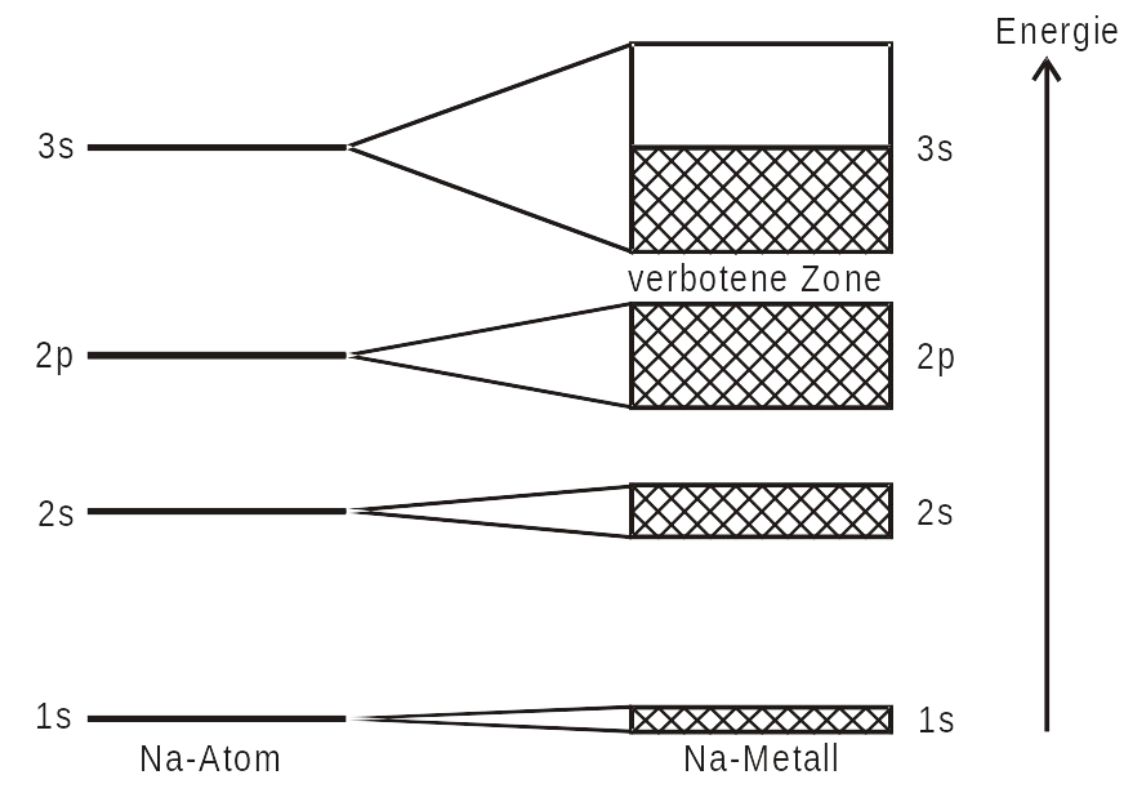
\includegraphics[height=6cm]{Energiebandmodell.png}
    \caption{Darstellung des Energiebandmodells am Beispiel von Natrium \cite{Versuchsanleitung_v511}.}
    \label{fig:Energiebandmodell}
\end{figure}

\noindent Wird nun die Beispielstruktur eines Natrium-Metalls betrachtet, so sind jeweils das 1s-, 2s und 2p-Band wegen der 
zugrundeliegenden Elektronenkonfiguration von Natrium voll besetzt. Die sich hierin befindenen Elektronen können weder 
Energie aufnehmen noch abgeben, weshalb sie insbesondere keine dynamische Reaktion auf ein externes elektrsiches Feld zeigen.
Dies gilt jedoch nicht für das ungepaarte Elektron im 3s-Band. Dieses Band verfügt über einen freien Platz für ein Elektron 
mit entgegengesetztem Spin, weshalb das Elektron bei Anlegen eines elektrischen Feldes in Feldrichtung beschleunigt werden 
und einen makroskopischen Strom erzeugen. Das nur teiweise bestzte Energieband ist somit ausschlaggebend für die hohe 
elektrische Leitfähigkeit von Metallen und wird daher auch als \emph{Leitfähigkeitsband} bezeichnet.\\

\noindent Nun liegt die Aufgabe jedoch darin mathematische Korrealtionen zwischen physikalisch messbaren Größen und mikroskopischen 
Parametern zu finden, um Aussagen über die Bewegungseigenschaften der Leitungselektronen zu treffen. In einem realen Kristall 
sind Fehlstellen im Gitter oder Struturdefekte Gründe für die Zusammenstöße zwischen Leitungselektronen und anderen Atomen.
Dementsprechend könnte es von Interesse sein, konkrete Aussagen über jene gemittelte Zeit zu treffen, die zwischen zwei 
Zusammenstößen vergeht. Dieses Intervall wird im Folgenden als Flugzeit $\tau$ bezeichnet. Bei einem extern angelegten elektrischen 
Feld der Feldstärke $\vec{E}$ beschleunigt ein Elektron während der Zeit $\bar{\tau}$ gleichmäßig mit 

\begin{equation*}
    \vec{b} = -\frac{e_0}{m_0}\vec{E}.
\end{equation*}

\noindent Hierbei steht $-e_0$ für die Elemenentarladung und $m_0$ für die Ruhemasse eines Elektrons. Die zugehörige
Geschwindigkeitsänderung $\increment{}\vec{v}$ während der Zeit $\bar{\tau}$ berechnet sich über 

\begin{equation}
\label{eqn:velocity}
    \increment{}\vec{v} = \vec{b}\bar{\tau} = -\frac{e_0}{m_0}\vec{E}\bar{\tau}.
\end{equation}

\noindent Aufgrund der räumlich zufälligen Streuung der Elektronen nach jedem Stoß ist die mittlere Geschwindigkeit 
eines Elektrons in Richtung des elektrischen Feldes zu Beginn der Flugzeit null. Daher wird die sogenannte mittlere 
Driftgeschwindigkeit $\vec{v_\text{d}}$ mit 

\begin{equation}
\label{eqn:drift}
    \vec{v}_\text{d} = \frac{1}{2}\increment{}\vec{v}.
\end{equation}

\noindent Die Stromdichte $\vec{j}$ eines Leiters beschreibt den Strom pro Querschnittsfläche und wird berechnet durch

\begin{equation}
\label{eqn:Stromdichte}
    \vec{j} = -n\vec{\bar{v}_\text{d}}e_0.
\end{equation}

\noindent Dabei steht $n$ für die Ladungsträgerdichte (Elektronen pro Volumen). Diese kann mittels der Gleichungen 
\eqref{eqn:velocity} und \eqref{eqn:drift} ausgedrückt werden als 

\begin{equation}
\label{eqn:Stromdichte}
    \vec{j} = \frac{e_{0}²}{2m_0}n\bar{\tau}\vec{E}.
\end{equation}

\noindent Bei einem homogenen Leiter der Länge $L$ und Querschnitt $Q$ lässt sich die Stromdichte schreiben als 
$j = \sfrac{I}{Q}$ und das elektrische Feld ersetzen durch $E = \sfrac{U}{L}$. Somit nimmt die Gleichung eine Form
an, welche dem \emph{Ohm'schen Gesetz} ähnelt:

\begin{equation*}
    I = \frac{e_{0}²}{2m_0}n\bar{\tau}\frac{Q}{L}U 
\end{equation*}

\noindent Hierbei lässt sich die elektrische Leitfähigkeit S gegeben durch 

\begin{equation}
\label{eqn:ELS}
    S = \frac{e_{0}²}{2m_0}n\bar{\tau}\frac{Q}{L}
\end{equation}

\noindent und der elektrische Widerstand $R = \sfrac{1}{S}$ erkennen.\\

\noindent Sowohl die geometrischen Abmessungen als auch der elektrische Widerstand sind einfach zu messende Größen. 
Es befinden sich mit Blick auf Gleichung \eqref{eqn:ELS} somit noch zwei mikroskopische Größen in der Rechnung.\\

\noindent Ein anderer Ausdruck für diese Parameter lässt sich durch den \emph{Hall-Effekt} finden. Hierzu muss die in der folgenden 
Abbildung dargestellte Versuchsanordnung betrachtet werden.

\begin{figure}[H]
    \centering 
    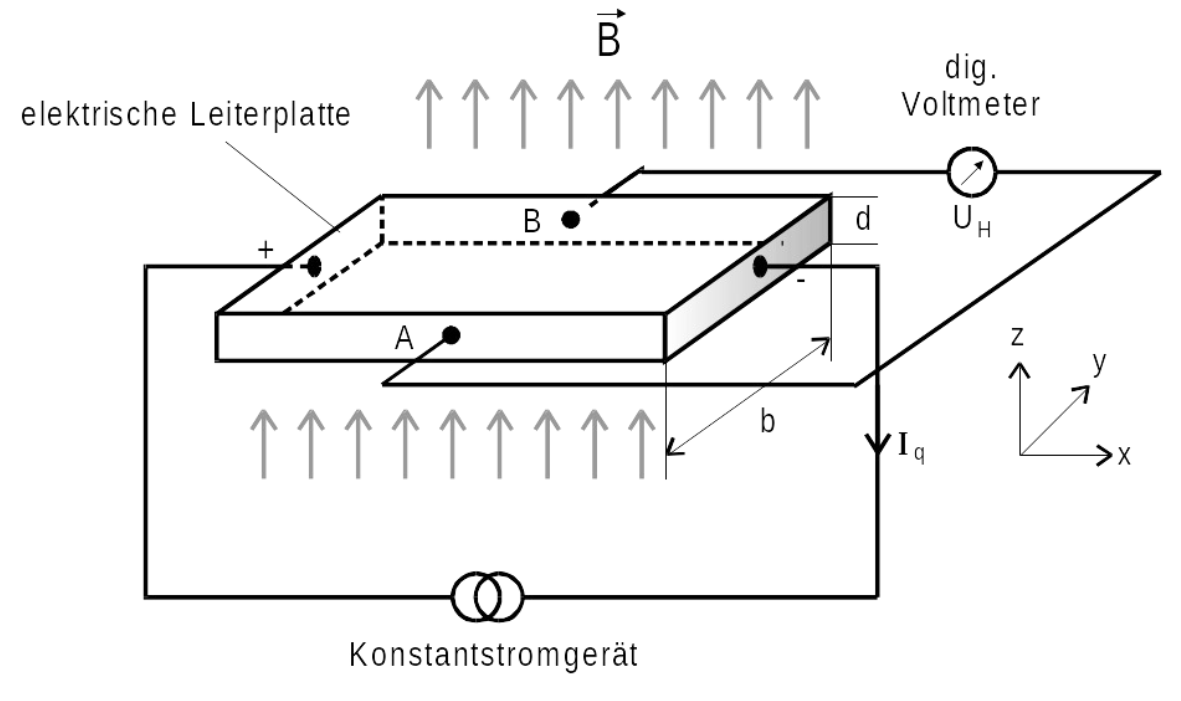
\includegraphics[height=7cm]{Hall-Effekt.png}
    \caption{Versuchsanordnung zum Hall-Effekt \cite{Versuchsanleitung_v511}}
    \label{fig:Hall-Effekt}
\end{figure}

\noindent Grundelement der Versuchsapparatur ist eine stromdurchflossene homogene Leiterplatte der Dicke $d$ und Breite $b$.
Die Oberfläche der Leiterplatte steht senkrecht zu einem magnetischen Feld. Bei Einschalten des B-Feldes lässt an den 
seitlichen Punkten A und B der Leiterplatte eine Spannung $U_\text{H}$, die \emph{Hall-Spannung} abgreifen.
Dieses Phänomen ist auf die Lorentz-Kraft\footnote{Die Lorentz-Kraft wirkt auf bewegte Ladungsträger im magnetischen Feld.}
zurückzuführen. Da sich die Elektronen in negative x-Richtung mit Driftgeschwindigkeit bewegen, lautet der 
Betrag der Lorentz-Kraft 

\begin{equation*}
    F_\text{L} = e_{0}\bar{v}_\text{d}B. 
\end{equation*}

\noindent Die somit entstehende Ladungsdifferenz sorgt für ein elektrisches Feld $E_\text{Y}$, welches der 
Elektronenbewegung entgegenwirkt und so groß wird, dass es zu einem Kräftegleichgewicht kommt:

\begin{equation*}
    e_{0}E_\text{Y} = e_{0}\bar{v}_\text{d}B 
\end{equation*}

\noindent Nach der Abbildung \ref{fig:Hall-Effekt} und Gleichung \eqref{eqn:Stromdichte} lässt sich schließlich
folgender Ausdruck für die Hall-Spannung finden 

\begin{equation*}
    U_\text{H} = -\frac{1}{ne_0}\frac{B\cdot{}I_\text{q}}{d}
\end{equation*}

\noindent Nun ist es möglich anhand des elektrischen Widerstandes und der Hall-Spannung die 
mikroskopischen Parameter $\bar{\tau}$ und $n$ zu bestimmen.\\

\noindent Das räumliche Analogon der Flugzeit ist die mittlere freie Weglänge $\bar{l}$, welche die 
die Entfernung beschreibt, die ein Elektron im Mittel zwischen zwei Zusammenstößen zurücklegt.
Daher gilt die Beziehung

\begin{equation}
\label{eqn:Weglaenge}
    \bar{l} = \bar{\tau}\cdot|v|,
\end{equation}

\noindent wobei $|v|$ die Totalgeschwindigkeit der Elektronen beschreibt. In Anlehung an die ideale 
Gastheorie ist die Temperatur eines Stoffes ein Maß für die mittlere kinetische Energie. Übertragen auf die 
Leitungselektronen in einem Festkörper gilt dementsprechend

\begin{equation*}
    E_\text{kin} = \frac{3}{2}kT.
\end{equation*}

\noindent Daraus ergibt sich eine mittlere Totalgeschwindigkeit $|v_\text{kl}| = \sqrt{\sfrac{3kT}{m_0}}$.\\

\noindent Die Wahrscheinlichkeitsverteilung der Energiewerte der Elektronen kann jedoch aufgrund des Pauli-Verbotes
nicht durch eine Maxwell-Boltzmann-Statistik beschrieben, sondern ist durch die \textbf{Fermi-Dirac-Verteilung} 
gegeben. Die Wahrscheinlichkeit $f(E)$ ein Elektron mit der Energie $E + \symup{d}E$ zu treffen 
beträgt hierbei 

\begin{equation*}
    f(E)\symup{d}E = \frac{1}{\exp{\left(\frac{E-E_\text{f}}{kT}\right)}+1}
\end{equation*}

\noindent mit der sogenannten \emph{Fermi-Energie}\footnote{Sie bezeichnet den Wert der energiereichsten Elektronen
am absoluten Nullpunkt.} $E_\text{F}$. Diese Energie ist essenziell für die Berechnung der Totalgeschwindigkeit, da nur jene 
Elektronen mit $E = E_\text{F}$ eine wesentliche Rolle für die Leitfähigkeit spielen. Ein geeignetere Abschätzung für 
den Wert der Totalgeschwindigkeit ist somit 

\begin{equation*}
    |\bar{v}| \approx \sqrt{\frac{2E_\text{F}}{m_0}}
\end{equation*}

\noindent mit 

\begin{equation*}
    E_\text{F} = \frac{h²}{2m_0}\sqrt[3]{\left(\frac{3}{8\pi}n\right)²}.
\end{equation*}

\noindent Mit Rückbezug zu Gleichung \eqref{eqn:Weglaenge} ist demnach 

\begin{equation*}
    \bar{l} = \bar{\tau}\sqrt{\frac{2E_\text{F}}{m_0}}.
\end{equation*}

\noindent Eine letzte mikroskopische Größe ist der Proportionalitätsfaktor zwischen der Driftgeschwindigkeit und der
elektrischen Feldstärke. Dieser Parameter wird als \emph{Beweglichkeit} $\mu$ und lässt sich aus der Flugzeit
$\bar{\tau}$ berechnen.\\

\noindent Neben dem soeben präsentierten Phänomen der Elektrizitätsleitung in Metallen
über Leitungselektronen in nicht voll besetzten Energiebändern existiert eine weitere Art und Weise der Leitfähigkeit.
Bei Überlappung zweier Energiebänder kann es gelegentlich zu Übergängen von Elektronen vom unteren in das 
obere Energieband kommen. Die so entstehenden, ortsveränderlichen Löcher bewegen sich unter Einwirkung eines äußeren 
E-Feldes und verhalten sich dabei wie positive Ladungen. Die dadurch hervorgerufenen Hall-Spannung besitzt ein 
umgekehrtes Vorzeichen, weshalb auch von einem \emph{anomalen Hall-Effekt} gesprochen wird. 

\section{Vorbereitung}


\section{Fehlerrechnung}
\end{document}